\subsection{Portfolio: The Seven Models Combined}
\label{Subsection:Portfolio}

A trader would not run one of these agents. They would run all seven, which is a different question from how each performs alone, because what matters for a portfolio is not only what each component returns but whether they lose money at the same time.

The seven published models are combined by giving each a seventh of the capital at the start of the window and never rebalancing. Writing $E_p(t)$ for the equity of pair $p$ at time $t$, the portfolio is

\begin{equation}
V(t) = \frac{1}{7} \sum_{p} \frac{E_p(t)}{E_p(0)}
\label{Equation:Portfolio}
\end{equation}

The total return of such a portfolio is the mean of its components by construction, so the return is not the interesting part. The risk is. Table~\ref{Tables:Portfolio} sets the portfolio against the average of the seven pairs taken separately.

\begin{table}[htb!]
\centering
\footnotesize
\begin{tabular}{@{}lrrl@{}}
\toprule
\textbf{Measure} & \textbf{Portfolio} & \textbf{Mean of the seven} & \textbf{Effect} \\
\midrule
Total return & $+91.3\%$ & $+91.3\%$ & Equal by construction \\
Annualised return & $+6.07\%$ & $+6.07\%$ & Equal by construction \\
\addlinespace
Maximum drawdown & $\mathbf{15.9\%}$ & $34.5\%$ & More than halved \\
Sharpe ratio & $\mathbf{0.632}$ & $0.451$ & Above all but USD/CHF \\
Sortino ratio & $0.906$ & $0.685$ & Improved \\
Calmar ratio & $0.381$ & $0.194$ & Nearly doubled \\
Sterling ratio & $1.059$ & $0.670$ & Improved \\
\addlinespace
Mean correlation & \multicolumn{2}{c}{$+0.062$ across all 21 pairings} & Near independence \\
\bottomrule
\end{tabular}
\caption{The equal-weight portfolio of Equation~\ref{Equation:Portfolio} against the average of its seven components. Return is identical by construction, so the whole effect is on risk.}
\label{Tables:Portfolio}
\end{table}

The maximum drawdown falls from an average of $34.5\%$ to $15.9\%$, and the Sharpe ratio rises from an average of $0.451$ to $0.632$, above every individual pair except USD/CHF. The same return is delivered with less than half the worst loss.

\begin{figure}[htb!]
\centering
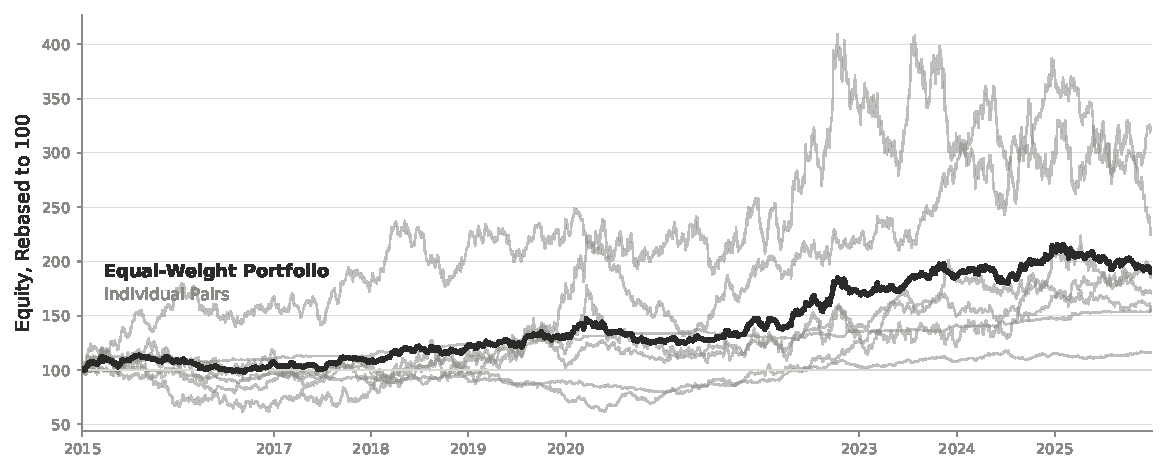
\includegraphics[width=\textwidth]{Images/PortfolioEquity.pdf}
\caption{The equal-weight portfolio against its seven components, all rebased to 100. The portfolio is smoother than any component because the components do not fall together.}
\label{Figure:PortfolioEquity}
\end{figure}

The reason is in Figure~\ref{Figure:Correlation}. The mean correlation between the daily returns of any two of the seven models is $+0.062$, and no pair of models exceeds $+0.46$. Three pairings are negative. These are seven agents trained by the same procedure on seven instruments that are themselves correlated, all sharing the US Dollar on one side, and yet their profits and losses arrive at different times. That is a consequence of the design: each agent learned the timing of its own market, so what they have in common is a method rather than a position.

\begin{figure}[htb!]
\centering
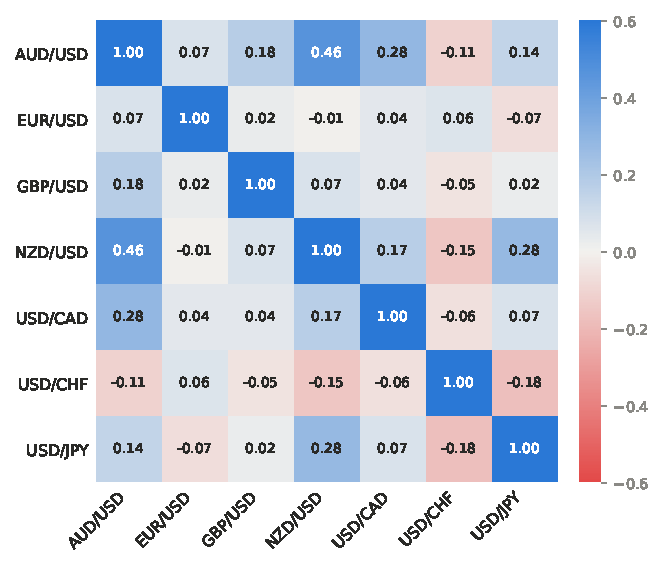
\includegraphics[width=0.68\textwidth]{Images/Correlation.pdf}
\caption{Correlation between the daily returns of the seven agents over the evaluation window. The mean of the off-diagonal entries is $+0.062$.}
\label{Figure:Correlation}
\end{figure}

Two qualifications belong with this result. The components do not all run at the same position size, as Section~\ref{Subsection:EvaluationProtocol} states, so the portfolio is the combination as published rather than a risk-parity allocation; equalising the sizes would change the weights but not the correlation structure that produces the benefit. And the portfolio inherits the limitation of its components: in the held-out year of Section~\ref{Subsection:OutOfSample} it returns $-9.8\%$, better than five of the seven pairs and worse than two, which is what an average should do when most of its components fall together for a reason they share.